% \section{Ferramentas} \label{sec:tools}
O protótipo foi equipado com um teclado LCD e três LEDs distintos; sendo o uso do teclado pela necessidade de atualização das crenças do agente monitor, responsáveis pela quantificação dos níveis de SpO$_2$ no sangue. Ademais, o componente também possui saída de dados por meio do visor LCD, para constatação dos dados exibidos na ChonIDE. Os LEDs foram escolhidos para identificar o status do hardware ao carregar o firmware compilado.
A escolha desse ferramental se deu pelo seu baixo custo e amplo suporte aos componentes, tornando a experimentação viável. O aparato descrito pode ser observado na Figura~\ref{fig:fig5}

\begin{figure}[H]
  \centering
  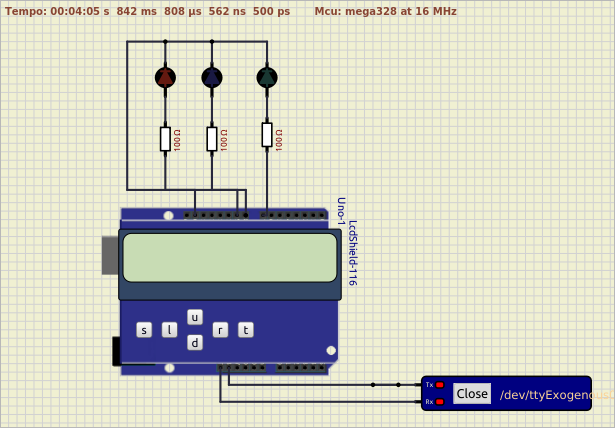
\includegraphics[width=0.7\textwidth]{assets/img/Oximeter.png}
  \caption{Protótipo do Oxímetro.}
  \label{fig:fig5}
\end{figure}

Já a parte lógica do projeto foi construída em \textit{AgentSpeak} na ChonIDE, para integração com o microcontrolador Arduino, por meio do Javino; durante a compilação do firmware escrito em ArduINO. Oximeter, projeto criado na ChonIDE para esta pesquisa, foi arquitetado seguindo o paradigma Multi-Agente, sendo constituído de quatro camadas de responsabilidade compostas por um agente cada. Assim, há melhor manutenção e escalabilidade ao projeto, seguindo os preceitos arquiteturais do ARGO \cite{pantoja2016argo}.

% \begin{figure}[H]
%   \centering
%   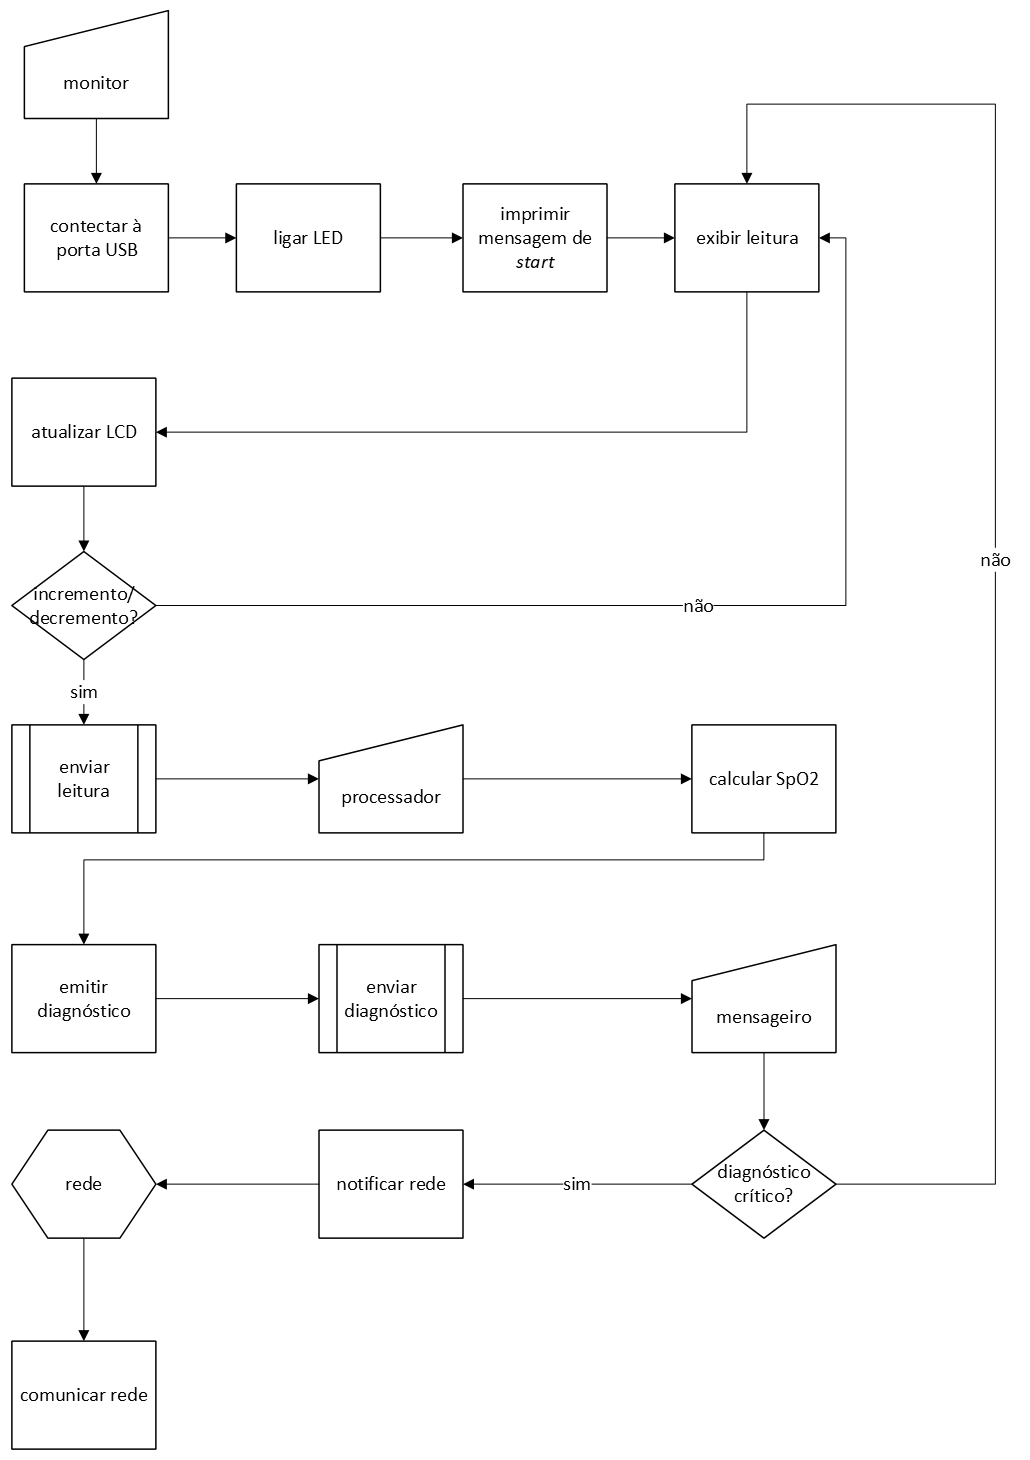
\includegraphics[width=0.9\textwidth]{assets/img/diagrama.png}
%   \caption{Arquitetura Conceitual}
%   \label{fig:fig4}
% \end{figure}